\documentclass[titlepage,landscape]{seminar}
\usepackage{url}
\usepackage{graphicx}
\usepackage[pdftex]{color}
\usepackage{hyperref}
\usepackage{epstopdf}
\usepackage{slides}

\newcommand{\frack}{\frac{1}{k}}
\newcommand{\quarter}{\frac{1}{4}}

\begin{document}

\myslide{
\[
P(\hbox{$j$ $A_1$ in offspring $|$ $i$ $A_1$ in parents}) =
{2N \choose j}\left(\frac{i}{2N}\right)\left(1 - \frac{i}{2N}\right)
\]
\vfil
\[
\hbox{Var}(p_{t+1}) = \frac{p_t(1-p_t)}{2N}
\]
}

\myslide{
\begin{eqnarray*}
f_{t+1} &=& \mbox{Prob. ibd from preceding generation} \\
        &&  + (\mbox{Prob. not ibd from prec. gen.}) \times (\mbox{Prob. ibd from
          earlier gen.}) \\
   &=& \frac{1}{2N} + \left(1 - \frac{1}{2N}\right)f_t
\end{eqnarray*}
\vfil
\[
f_{t+1} = 1 - \left(1 - \frac{1}{2N}\right)^t(1-f_0)
\]
}

\myslide{
\[
Var(p_{t+1}) = \frac{p_t(1-p_t)}{2N} \quad.
\]
\vfil
\[
N_e^{(v)} = \frac{p(1-p)}{2\widehat{Var}(p)}
\]
}

\myslide{
\[
f_{t+1}
   = \frac{1}{2N} + \left(1 - \frac{1}{2N}\right)f_t
\]
\vfil
\[
N_e^{(f)} = \frac{1 - \hat f_t}{2(\hat f_{t+1} - \hat f_t)}
\]
\vfil
Assume $\hat f_t = 0$
\[
N_e^{(f)} = \frac{1}{2\hat f_{t+1}}
\]
}

\myslide{
\begin{eqnarray*}
f_{t+1} &=& \left(1-\frac{1}{2N_t}\right)f_t + \frac{1}{2N_t} \\
1 - f_{t+1} &=& \left(1-\frac{1}{2N_t}\right)(1-f_t) \\
1 - f_{t+K} &=&
\left(\prod_{i=1}^K\left(1-\frac{1}{2N_{t+i}}\right)\right)(1-f_t) \quad .
\end{eqnarray*}
If the population size were constant
\begin{eqnarray*}
\left(\prod_{i=1}^K\left(1-\frac{1}{2N_{t+i}}\right)\right) &=&
\left(1 - \frac{1}{2N_e^{(f)}}\right)^K \\
\sum_{i=1}^K\log\left(1-\frac{1}{2N_{t+i}}\right) &=&
K\log\left(1 - \frac{1}{2N_e^{(f)}}\right) 
\end{eqnarray*}
}

\myslide{
AWKF: If $x$ is small,
\[
\log(1 - x) \approx -x
\]
\vfill
\begin{eqnarray*}
\sum_{i=1}^K\log\left(1-\frac{1}{2N_{t+i}}\right) &=&
K\log\left(1 - \frac{1}{2N_e^{(f)}}\right) \\
\sum_{i=1}^K-\frac{1}{2N_{t+i}}
  &\approx& K\left(-\frac{1}{2N_e^{(f)}}\right) \\
\frac{K}{N_e^{(f)}} &=& \sum_{i=1}^K\frac{1}{N_{t+i}} \\
\frac{1}{N_e^{(f)}} &=& \left(\frac{1}{K}\right)\sum_{i=1}^K\frac{1}{N_{t+i}} \\
N_e^{(f)} &=& \left(\left(\frac{1}{K}\right)
                    \sum_{i=1}^K\frac{1}{N_{t+i}}\right)^{-1}
\end{eqnarray*}
}

\myslide{
\begin{eqnarray*}
f_{t+1} &=& \left(\half\right) \left(\frac{N-1}{2N-1}\right)
            \left(\frac{1}{2N_f}\right) +
            \left(\half\right) \left(\frac{N-1}{2N-1}\right)
            \left(\frac{1}{2N_m}\right) \\
        &=& \left(\half\right) \left(\frac{N-1}{2N-1}\right)
            \left(\frac{1}{2N_f} + \frac{1}{2N_m}\right) \\
        &\approx& \left(\quarter\right)
            \left(\frac{2N_m + 2N_f}{4N_fN_m}\right) \\
        &=& \left(\half\right)
            \left(\frac{N_m + N_f}{4N_fN_m}\right) \\
N_e^{(f)} &\approx& \frac{4N_fN_m}{N_f + N_m} \quad 
\end{eqnarray*}
}

\myslide{
\[
N_e^{(f)} = \frac{2N - 1}{1 + \frac{V_k}{2}} \quad ,
\]
\vfill
\begin{itemize}

\item $N_e^{(f)} < N$ if $V_k > 2(1 - 1/N)$ and

\item $N_e^{(f)} > N$ if $V_k < 2(1 - 1/N)$.

\end{itemize}
}

\myslide{
\[
f_{t+1} = \left(\left(\frac{1}{2N}\right) +
          \left(1 - \frac{1}{2N}\right)f_t\right)(1-\mu)^2
\]
}

\myslide{
\begin{eqnarray*}
\hat f &=& \left(\left(\frac{1}{2N}\right) +
          \left(1 - \frac{1}{2N}\right)\hat f\right)(1-\mu)^2 \\
\hat f\left(1 -
\left(1 - \frac{1}{2N}\right)(1-\mu)^2\right)
       &=& \left(\frac{1}{2N}\right)(1-\mu)^2 \\
\hat f &=& \frac{\left(\frac{1}{2N}\right)(1-\mu)^2}
           {1 -\left(1 - \frac{1}{2N}\right)(1-\mu)^2} \\
       &\approx& \frac{1 - 2\mu}
           {2N\left(1 - \left(1 - \frac{1}{2N}\right)(1-2\mu)\right)} \\
       &=& \frac{1 - 2\mu}
           {2N\left(1 - 1 + \frac{1}{2N} + 2\mu -
            \frac{2\mu}{2N}\right)} \\
       &=& \frac{1 - 2\mu}{1 + 4N\mu - 2\mu} \\
       &\approx& \frac{1}{4N\mu + 1}
\end{eqnarray*}
}

\myslide{
\begin{center}
\resizebox{!}{\textheight}{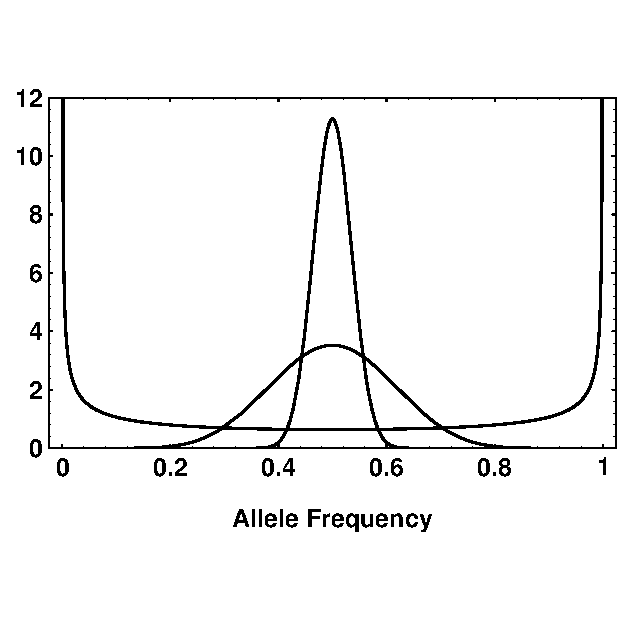
\includegraphics{mutation.eps}}
\end{center}
}

\myslide{
\[
f_{t+1} = \left(\left(\frac{1}{2N}\right) +
          \left(1 - \frac{1}{2N}\right)f_t\right)(1-m)^2
\]
\vfill
\[
\hat f \approx \frac{1}{4Nm + 1}
\]
}

\end{document}

